% =====================================================================
% LeBlanc — paper skeleton.
%
% READ THIS FIRST
% ---------------
% This document is a TEMPLATE showing what the paper will look like. Every
% quantitative value in it is wrapped in \PLACEHOLDER{} and typesets in red,
% because NO REAL RESULTS EXIST YET — the full experiment (M4) has not been run.
% Do not circulate this as a findings document. Do not let a placeholder survive
% into a submitted draft: \PLACEHOLDERSREMAIN below counts them for you, and the
% title page prints a DRAFT banner while any remain.
%
% Filling it in: run `python analysis/rq_analysis.py`, then either copy values
% from analysis/output/SUMMARY.md or \input the generated tables directly, e.g.
%     \input{../analysis/output/tables/rq1.tex}
% The project rule (docs/04_PAPER.md) is absolute: if a number is in this paper,
% it came out of analysis/output/. Nothing is hand-computed.
%
% Build: pdflatex leblanc_paper.tex && pdflatex leblanc_paper.tex
% =====================================================================
\documentclass[10pt,conference]{article}

\usepackage[margin=1in]{geometry}
\usepackage{times}
\usepackage{graphicx}
\usepackage{booktabs}
\usepackage{xcolor}
\usepackage{tikz}
\usetikzlibrary{shapes.geometric, arrows.meta, positioning, fit, backgrounds}
\usepackage{float}
\usepackage{hyperref}
\hypersetup{colorlinks=true, linkcolor=black, citecolor=black, urlcolor=blue}

\definecolor{accent}{HTML}{2A78D6}
\definecolor{midgray}{HTML}{52514E}
\definecolor{lightgray}{HTML}{F4F4F2}
\definecolor{placeholderred}{HTML}{C0392B}

% Every unfilled number wears this. Impossible to miss, impossible to submit by
% accident, and greppable: \grep '\\PLACEHOLDER' leblanc_paper.tex
\newcommand{\PLACEHOLDER}[1]{{\color{placeholderred}\textbf{[#1]}}}
\newcommand{\TODO}[1]{{\color{placeholderred}\textit{[TODO: #1]}}}

\title{\vspace{-1.5em}
  {\color{placeholderred}\large DRAFT SKELETON --- CONTAINS NO REAL RESULTS}\\[0.6em]
  Does Security Scaffolding Still Matter?\\
  Prompt Enrichment and Iterative Repair Across LLM Generations}

\author{
  Banerjee, Kumari, Ranjan, Soni\\
  \textit{Department of Information Technology}\\
  \textit{K.\,J.\ Somaiya School of Engineering}\\
  \small Supervisor: Prof.\ Deepti Patole
}
\date{}

\begin{document}
\maketitle

\begin{center}
\fcolorbox{placeholderred}{white}{\parbox{0.92\textwidth}{\small\color{placeholderred}
\textbf{Template notice.} This is the paper's structure, not its findings. Every
value shown as \PLACEHOLDER{like this} is a slot awaiting a number generated by
\texttt{analysis/rq\_analysis.py} from the run database. The experiment described
in Section~\ref{sec:design} has not yet been executed at full scale.}}
\end{center}

\begin{abstract}
Large language models are now routinely used to generate application code, and a
well-established line of work (2022--2024) showed that two inference-time
interventions measurably improve the security of that code: warning the model
about relevant weaknesses \emph{before} generation (prompt enrichment), and
feeding static-analysis findings back for correction \emph{after} it
(scanner-guided repair). Those results were obtained on the models of that era.
We ask whether they still hold. We evaluate \PLACEHOLDER{N} models spanning
\PLACEHOLDER{K} capability tiers on \PLACEHOLDER{50} security-sensitive Python
tasks under three conditions (unaided, enriched, enriched\,+\,repaired), with
\PLACEHOLDER{3} repetitions per cell, judging every output with two independent
static analysers \emph{and} executing it against per-task functional tests.
We find that baseline vulnerability rates \PLACEHOLDER{rise/fall/hold} across
tiers (\PLACEHOLDER{x}\% to \PLACEHOLDER{y}\%), that enrichment
\PLACEHOLDER{does/does not} retain its benefit on current models
(\(\Delta\)\PLACEHOLDER{z}\,pp), and---our sharpest result---that
\PLACEHOLDER{r}\% of repairs a scanner certifies as clean no longer pass their
functional tests, a failure mode invisible to every prior evaluation of
scanner-guided repair. We release the harness, the frozen task set, and the
complete run database.
\end{abstract}

% =====================================================================
\section{Introduction}

Pearce et al.~\cite{pearce2022asleep} reported that roughly 40\% of code
generated by GitHub Copilot in security-relevant scenarios contained a weakness.
The finding shaped a research programme: if models write insecure code, either
teach them not to (fine-tuning, constrained decoding) or catch it at inference
time (enrichment, repair). The inference-time branch is the practically important
one, because it is the only branch available to the overwhelming majority of
practitioners, who consume models through an API and will never touch a weight or
a logit.

That branch's evidence base, however, predates the current model generation.
SecuCoGen~\cite{wang2024secucogen} demonstrated CWE-aware prompting on
GPT-3.5-class models; HexaCoder~\cite{hajipour2024hexacoder} and
SVEN~\cite{he2023sven} showed oracle-guided repair, but as training-time
procedures; the Copilot replication study~\cite{majdinasab2023replication}
documented that a single assistant's security behaviour drifts substantially
between versions. Models have since improved markedly at producing plausible,
idiomatic code unaided. Whether the scaffolding built for weaker models still
earns its place is an empirical question that, to our knowledge, nobody has
re-asked with a consistent pipeline across model tiers.

A second gap is sharper. Every evaluation of scanner-guided repair we are aware
of scores repair by re-running the scanner: if the analyser stops complaining,
the repair succeeded. That criterion cannot distinguish a genuine fix from a
deletion. A model that resolves a SQL-injection finding by removing the database
call satisfies the scanner completely. CODEGUARD+~\cite{fu2024constrained} and
CodeSecEval~\cite{wang2024codeseceval} both argue that security must be judged
alongside functional correctness, and both measure the two together for
\emph{generation}. Neither measures it inside a live, multi-round repair loop,
which is exactly where the incentive to silently delete functionality is
strongest.

\noindent\textbf{Contributions.}
\begin{itemize}\itemsep2pt
  \item A quantification of how much prompt enrichment and scanner-guided repair
        still change security outcomes across \PLACEHOLDER{K} model tiers, using
        one pipeline, one task set, and one judge (\S\ref{sec:rq1}--\S\ref{sec:rq3}).
  \item A residual-risk catalogue: the weakness categories that survive
        \emph{full} scaffolding on current models (\S\ref{sec:rq4}) --- the
        practitioner-facing result.
  \item \textbf{Repair inflation:} the first measurement, to our knowledge, of how
        often scanner-certified repairs are functionally broken, measured inside
        the repair loop and against a never-repaired control
        (\S\ref{sec:rq5}).
  \item An open harness, a frozen \PLACEHOLDER{50}-task set with provenance, and
        the full run database, such that every number here is regenerable by one
        command.
\end{itemize}

% =====================================================================
\section{Background and Related Work}

\paragraph{Insecure generation.} \TODO{Pearce et al.; Siddiq \& Santos'
SecurityEval; Yan et al.\ on self-generated hints. Establish the baseline rates
prior work reports, which our RQ1 re-measures.}

\paragraph{Prompt-level intervention.} \TODO{SecuCoGen's CWE-aware prompting;
Yan et al.'s self-generated and contextualised hints, including their finding
that imprecise hints can \emph{increase} vulnerability rates --- directly
relevant to our RQ2 discordant-pair analysis.}

\paragraph{Repair.} \TODO{HexaCoder's oracle-report-plus-hint format, which our
Engine C mirrors at inference time; SVEN; Pearce et al.\ on zero-shot repair.
Emphasise: all evaluate repair by re-scanning only.}

\paragraph{Security \emph{and} correctness.} \TODO{CODEGUARD+'s secure-pass@k;
CodeSecEval. This is the lineage our RQ5 extends from generation into the repair
loop.}

\paragraph{What we deliberately do not do.} Fine-tuning approaches
(LPO/DiSCo, HexaCoder's training stage) require weight access. We restrict
ourselves to what an API consumer can do, which is the population the result is
for.

% =====================================================================
\section{The LeBlanc Pipeline}

% LeBlanc v3 pipeline diagram — standalone TikZ figure, drop into any paper.
%
% Provenance: adapted from the TikZ figure in the (now-removed) April 2026
% VAPT mini-project report, corrected to the v3 pipeline: four engines, not
% three (Engine D — the functional-test honesty layer — did not exist in the
% version that diagram was drawn for), a 3-iteration repair cap (not 5), and
% the current 6-model fleet instead of the two-model Gemini/Llama pairing.
%
% Requires in the preamble:
%   \usepackage{tikz}
%   \usetikzlibrary{shapes.geometric, arrows.meta, positioning, fit, backgrounds}
%   \usepackage{float}
%   \definecolor{accent}{HTML}{2A78D6}
%   \definecolor{midgray}{HTML}{52514E}
%   \definecolor{lightgray}{HTML}{F4F4F2}
%
% Usage: % LeBlanc v3 pipeline diagram — standalone TikZ figure, drop into any paper.
%
% Provenance: adapted from the TikZ figure in the (now-removed) April 2026
% VAPT mini-project report, corrected to the v3 pipeline: four engines, not
% three (Engine D — the functional-test honesty layer — did not exist in the
% version that diagram was drawn for), a 3-iteration repair cap (not 5), and
% the current 6-model fleet instead of the two-model Gemini/Llama pairing.
%
% Requires in the preamble:
%   \usepackage{tikz}
%   \usetikzlibrary{shapes.geometric, arrows.meta, positioning, fit, backgrounds}
%   \usepackage{float}
%   \definecolor{accent}{HTML}{2A78D6}
%   \definecolor{midgray}{HTML}{52514E}
%   \definecolor{lightgray}{HTML}{F4F4F2}
%
% Usage: % LeBlanc v3 pipeline diagram — standalone TikZ figure, drop into any paper.
%
% Provenance: adapted from the TikZ figure in the (now-removed) April 2026
% VAPT mini-project report, corrected to the v3 pipeline: four engines, not
% three (Engine D — the functional-test honesty layer — did not exist in the
% version that diagram was drawn for), a 3-iteration repair cap (not 5), and
% the current 6-model fleet instead of the two-model Gemini/Llama pairing.
%
% Requires in the preamble:
%   \usepackage{tikz}
%   \usetikzlibrary{shapes.geometric, arrows.meta, positioning, fit, backgrounds}
%   \usepackage{float}
%   \definecolor{accent}{HTML}{2A78D6}
%   \definecolor{midgray}{HTML}{52514E}
%   \definecolor{lightgray}{HTML}{F4F4F2}
%
% Usage: \input{figures/pipeline_diagram.tex}

\begin{figure}[H]
\centering
\resizebox{\textwidth}{!}{%
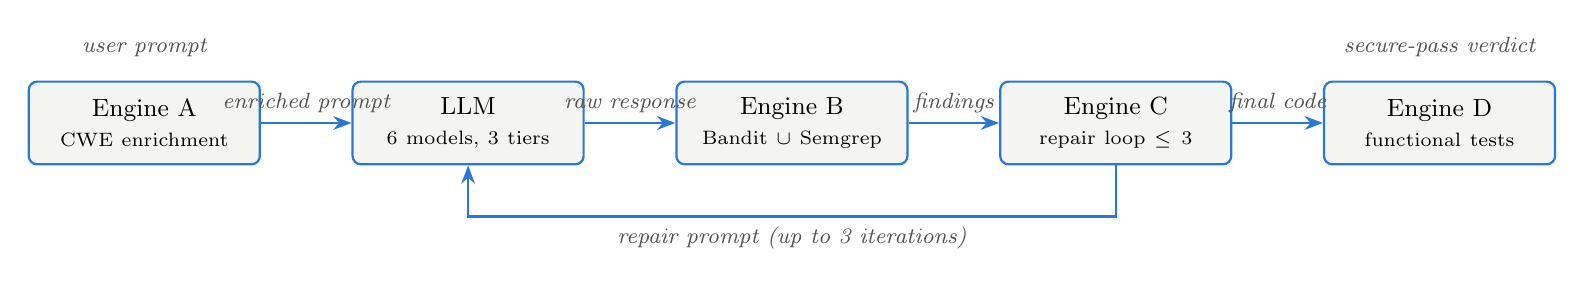
\begin{tikzpicture}[
  font=\small,
  box/.style={rectangle, rounded corners=3pt, draw=accent, thick,
              fill=lightgray, text width=2.7cm, align=center, minimum height=1.05cm},
  arrow/.style={-Stealth, thick, color=accent},
  lbl/.style={font=\footnotesize\itshape, color=midgray},
]

\node[box] (A) {Engine A\\{\scriptsize CWE enrichment}};
\node[box, right=1.15cm of A] (LLM) {LLM\\{\scriptsize 6 models, 3 tiers}};
\node[box, right=1.15cm of LLM] (B) {Engine B\\{\scriptsize Bandit $\cup$ Semgrep}};
\node[box, right=1.15cm of B] (C) {Engine C\\{\scriptsize repair loop $\leq 3$}};
\node[box, right=1.15cm of C] (D) {Engine D\\{\scriptsize functional tests}};

\draw[arrow] (A) -- (LLM) node[midway, above, lbl] {enriched prompt};
\draw[arrow] (LLM) -- (B) node[midway, above, lbl] {raw response};
\draw[arrow] (B) -- (C) node[midway, above, lbl] {findings};
\draw[arrow] (C) -- (D) node[midway, above, lbl] {final code};
\draw[arrow] (C.south) -- ++(0,-0.65) -| (LLM.south)
      node[near start, below, lbl] {repair prompt (up to 3 iterations)};

\node[above=0.18cm of A, lbl] {user prompt};
\node[above=0.18cm of D, lbl] {secure-pass verdict};
\end{tikzpicture}%
}
\caption{The LeBlanc v3 pipeline. Engine A injects CWE warnings before generation
(rule-based, no LLM call); Engine B scans the generated code with two independent
static analysers; Engine C feeds findings back to the \emph{same} model for up to
three repair rounds; Engine D executes the final code against per-prompt functional
tests, which is what makes a ``clean'' verdict falsifiable (RQ5).}
\label{fig:pipeline}
\end{figure}


\begin{figure}[H]
\centering
\resizebox{\textwidth}{!}{%
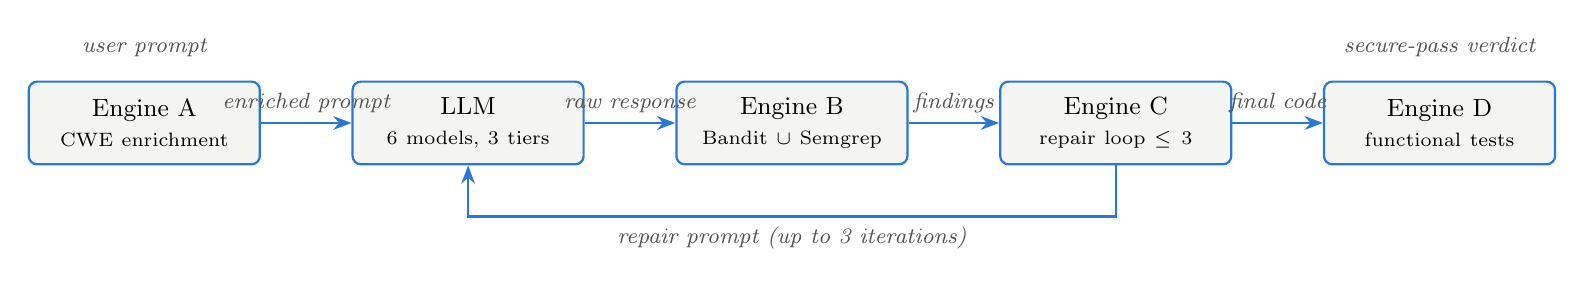
\begin{tikzpicture}[
  font=\small,
  box/.style={rectangle, rounded corners=3pt, draw=accent, thick,
              fill=lightgray, text width=2.7cm, align=center, minimum height=1.05cm},
  arrow/.style={-Stealth, thick, color=accent},
  lbl/.style={font=\footnotesize\itshape, color=midgray},
]

\node[box] (A) {Engine A\\{\scriptsize CWE enrichment}};
\node[box, right=1.15cm of A] (LLM) {LLM\\{\scriptsize 6 models, 3 tiers}};
\node[box, right=1.15cm of LLM] (B) {Engine B\\{\scriptsize Bandit $\cup$ Semgrep}};
\node[box, right=1.15cm of B] (C) {Engine C\\{\scriptsize repair loop $\leq 3$}};
\node[box, right=1.15cm of C] (D) {Engine D\\{\scriptsize functional tests}};

\draw[arrow] (A) -- (LLM) node[midway, above, lbl] {enriched prompt};
\draw[arrow] (LLM) -- (B) node[midway, above, lbl] {raw response};
\draw[arrow] (B) -- (C) node[midway, above, lbl] {findings};
\draw[arrow] (C) -- (D) node[midway, above, lbl] {final code};
\draw[arrow] (C.south) -- ++(0,-0.65) -| (LLM.south)
      node[near start, below, lbl] {repair prompt (up to 3 iterations)};

\node[above=0.18cm of A, lbl] {user prompt};
\node[above=0.18cm of D, lbl] {secure-pass verdict};
\end{tikzpicture}%
}
\caption{The LeBlanc v3 pipeline. Engine A injects CWE warnings before generation
(rule-based, no LLM call); Engine B scans the generated code with two independent
static analysers; Engine C feeds findings back to the \emph{same} model for up to
three repair rounds; Engine D executes the final code against per-prompt functional
tests, which is what makes a ``clean'' verdict falsifiable (RQ5).}
\label{fig:pipeline}
\end{figure}


\begin{figure}[H]
\centering
\resizebox{\textwidth}{!}{%
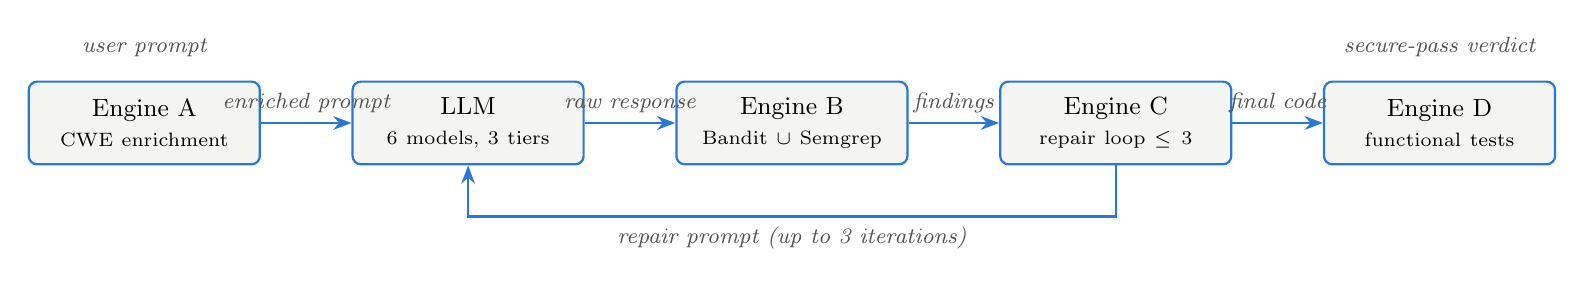
\begin{tikzpicture}[
  font=\small,
  box/.style={rectangle, rounded corners=3pt, draw=accent, thick,
              fill=lightgray, text width=2.7cm, align=center, minimum height=1.05cm},
  arrow/.style={-Stealth, thick, color=accent},
  lbl/.style={font=\footnotesize\itshape, color=midgray},
]

\node[box] (A) {Engine A\\{\scriptsize CWE enrichment}};
\node[box, right=1.15cm of A] (LLM) {LLM\\{\scriptsize 6 models, 3 tiers}};
\node[box, right=1.15cm of LLM] (B) {Engine B\\{\scriptsize Bandit $\cup$ Semgrep}};
\node[box, right=1.15cm of B] (C) {Engine C\\{\scriptsize repair loop $\leq 3$}};
\node[box, right=1.15cm of C] (D) {Engine D\\{\scriptsize functional tests}};

\draw[arrow] (A) -- (LLM) node[midway, above, lbl] {enriched prompt};
\draw[arrow] (LLM) -- (B) node[midway, above, lbl] {raw response};
\draw[arrow] (B) -- (C) node[midway, above, lbl] {findings};
\draw[arrow] (C) -- (D) node[midway, above, lbl] {final code};
\draw[arrow] (C.south) -- ++(0,-0.65) -| (LLM.south)
      node[near start, below, lbl] {repair prompt (up to 3 iterations)};

\node[above=0.18cm of A, lbl] {user prompt};
\node[above=0.18cm of D, lbl] {secure-pass verdict};
\end{tikzpicture}%
}
\caption{The LeBlanc v3 pipeline. Engine A injects CWE warnings before generation
(rule-based, no LLM call); Engine B scans the generated code with two independent
static analysers; Engine C feeds findings back to the \emph{same} model for up to
three repair rounds; Engine D executes the final code against per-prompt functional
tests, which is what makes a ``clean'' verdict falsifiable (RQ5).}
\label{fig:pipeline}
\end{figure}


\paragraph{Engine A --- enrichment.} Hybrid retrieval over a curated
\PLACEHOLDER{46}-entry CWE corpus: word-boundary lexical matching fused with
TF--IDF cosine similarity, top-\PLACEHOLDER{5} matches injected as explicit
warnings. Deterministic, offline, no model call --- the intervention costs
nothing at inference time, which is why the interesting question is whether it
still \emph{does} anything, not whether to deploy it.

\paragraph{Engine B --- the judge.} Bandit ($\ge$ medium severity) unioned with
Semgrep against a pinned local copy of the \texttt{p/python} pack
(\PLACEHOLDER{781} rules), deduplicated by line, CWE set, and a cross-tool
equivalence map. Pinning matters for reproducibility: a live registry pack
changes underneath a longitudinal experiment. Extraction and syntax failures are
their own outcome class and are never counted as clean.

\paragraph{Engine C --- repair.} Findings are formatted as a numbered list with
CWE context and returned to the \emph{same} model, with an explicit instruction
to preserve the public interface; the patched output is re-scanned. Capped at
\PLACEHOLDER{3} rounds. Non-convergence is reported, not discarded.

\paragraph{Engine D --- the honesty layer.} The final code is executed against
per-task \texttt{pytest} smoke tests in a sandboxed subprocess with no network,
using an offline harness that fakes MySQL, LDAP, and network I/O so that
database- and auth-shaped tasks remain testable. This is what makes
``clean'' falsifiable and what RQ5 rests on.

% =====================================================================
\section{Experimental Design}\label{sec:design}

\paragraph{Tasks.} \PLACEHOLDER{50} Python tasks, frozen before data collection:
\PLACEHOLDER{40} drawn from SecurityEval~\cite{siddiq2022securityeval} by
stratified selection (max 2 per CWE, provenance recorded per task) and
\PLACEHOLDER{10} written by the authors. The authored subset is a deliberate
hedge against benchmark contamination: SecurityEval has been public since 2022
and may appear in current training corpora, whereas the authored tasks have
not. \PLACEHOLDER{20} tasks carry functional tests validated against
hand-written secure reference solutions; exclusions are documented per task.

\paragraph{Models.} \PLACEHOLDER{6} models across \PLACEHOLDER{3} tiers and
\PLACEHOLDER{3} vendors. \TODO{Table of model, vendor, tier, and the
verify-at-build date. State plainly here that provider retirement of older
models mid-study means tiers separate capability/size, not calendar generation
--- see Threats to Validity.}

\paragraph{Conditions.} \texttt{plain} (no intervention), \texttt{enriched}
(Engine A only), \texttt{enriched\_repair} (Engines A and C).
\PLACEHOLDER{3} repetitions per cell at temperature \PLACEHOLDER{0.7}; the
non-zero temperature is deliberate, so repetitions are genuine independent
samples rather than near-duplicates.

\paragraph{Measures and statistics.} Vulnerability rate with Wilson 95\%
intervals; exact McNemar on paired plain/enriched outcomes; $\chi^2$ (Fisher for
small cells) across tiers; Mann--Whitney $U$ on iteration counts; and
\texttt{vuln $\sim$ mode * tier + category} as the headline logistic model.
Decision bands separating ``yes'', ``mixed'', and ``no'' were fixed in the
project's public documentation \emph{before} data collection and are applied
mechanically by the analysis script.

% =====================================================================
\section{Results}

\subsection{RQ1 --- Baseline vulnerability by tier}\label{sec:rq1}
\PLACEHOLDER{Insert analysis/output/tables/rq1.tex}
\PLACEHOLDER{Figure: figures/rq1\_baseline\_vr.png}

\noindent Unaided vulnerability rates range from \PLACEHOLDER{x}\% to
\PLACEHOLDER{y}\%. \TODO{State whether the ordering predicted by H1 holds, and
compare the absolute level against the $\approx$40\% Pearce et al.\ figure.}

\subsection{RQ2 --- Does enrichment still help?}\label{sec:rq2}
\PLACEHOLDER{Insert analysis/output/tables/rq2.tex}
\PLACEHOLDER{Figure: figures/rq2\_enrichment\_delta.png}

\noindent \TODO{Report $\Delta$E per model with McNemar $p$. Report discordant
pairs in both directions --- cases where enrichment turned clean output
vulnerable are a finding, not noise, and prior work reports the same effect for
imprecise hints.}

\subsection{RQ3 --- Does repair converge?}\label{sec:rq3}
\PLACEHOLDER{Insert analysis/output/tables/rq3.tex}
\PLACEHOLDER{Figure: figures/rq3\_convergence.png}

\noindent \TODO{Convergence rate and mean iterations per model; report the
non-convergence rate prominently rather than as a footnote.}

\subsection{RQ4 --- What survives full scaffolding}\label{sec:rq4}
\PLACEHOLDER{Figure: figures/rq4\_residual\_heatmap.png}

\noindent \TODO{Name the categories in the red band on current models. This is
the section a practitioner reads.}

\subsection{RQ5 --- Repair inflation}\label{sec:rq5}
\PLACEHOLDER{Insert analysis/output/tables/rq5.tex}
\PLACEHOLDER{Figure: figures/rq5\_repair\_inflation.png}

\noindent Of repairs the scanner certified clean, \PLACEHOLDER{r}\% fail their
functional tests. The comparison that supports the causal reading is against
never-repaired but equally scanner-clean code, which fails at \PLACEHOLDER{b}\%;
the difference attributable to repair is therefore \PLACEHOLDER{d}\,pp
(Fisher $p = $ \PLACEHOLDER{p}).

\TODO{Be disciplined about which sentence the data licenses. If the attributable
difference is small while both rates are high, the finding is ``scanner-clean
LLM code frequently does not work'' --- valuable, and a direct extension of the
secure-pass@k argument --- and is \emph{not} ``the repair loop breaks code''.
Write whichever one is true.}

\TODO{Include the qualitative coding of how repairs break functionality:
interface change, stub-out, dependency drift. One worked example per mode.}

% =====================================================================
\section{Threats to Validity}

\paragraph{Static-analysis error.} Our security verdict is Bandit $\cup$ Semgrep.
A stratified \PLACEHOLDER{10}\% sample was labelled TP/FP, giving a
false-positive rate of \PLACEHOLDER{f}\% \PLACEHOLDER{(with $\kappa =$ k, or:
single-annotator triage, no $\kappa$)}. \TODO{If the FP rate is high, say so here
and in the abstract, identify which rules drive it, and report rates with those
rules excluded as a sensitivity analysis.} We additionally report what fraction
of findings land on scaffolding the model volunteers (\texttt{app.run} blocks)
rather than on the requested function, since these inflate rates without
reflecting the task.

\paragraph{Tiers are not calendar generations.} Provider retirement of older
models during the study means our tiers separate capability and size among
concurrently available models. The generational claim is correspondingly weaker
and stated as such.

\paragraph{Smoke tests are not correctness.} Engine D establishes that code still
does its basic job; it does not establish full functional equivalence. It can
therefore only ever \emph{underestimate} breakage --- which makes RQ5 a lower
bound.

\paragraph{Scope.} Python only; \PLACEHOLDER{50} tasks; a 3-iteration repair cap;
one enrichment strategy. \PLACEHOLDER{20} of \PLACEHOLDER{50} tasks carry
functional tests, so RQ5's sample is smaller than RQ1--RQ4's and is reported at
its true $n$.

% =====================================================================
\section{Conclusion}

\TODO{Practitioner guidance, stated as a decision rule: for which model tiers and
which weakness categories does inference-time scaffolding still pay, and where is
it ceremony? Then the honest caveat about what a scanner-clean verdict does and
does not buy.}

\paragraph{Availability.} Harness, frozen task set, analysis scripts, and the
complete run database: \TODO{repository URL}.

% =====================================================================
\begin{thebibliography}{9}\small
\bibitem{pearce2022asleep} H.~Pearce et al., ``Asleep at the Keyboard? Assessing
  the Security of GitHub Copilot's Code Contributions,'' \emph{IEEE S\&P}, 2022.
\bibitem{siddiq2022securityeval} M.~L.~Siddiq and J.~C.~S.~Santos,
  ``SecurityEval Dataset,'' \emph{MSR4P\&S}, 2022.
\bibitem{wang2024secucogen} J.~Wang et al., ``Enhancing Large Language Models for
  Secure Code Generation: A Dataset-driven Study on Vulnerability Mitigation,''
  2024.
\bibitem{wang2024codeseceval} J.~Wang et al., ``Is Your AI-Generated Code Really
  Safe? Evaluating LLMs on Secure Code Generation with CodeSecEval,'' 2024.
\bibitem{fu2024constrained} Y.~Fu et al., ``Constrained Decoding for Secure Code
  Generation,'' 2024.
\bibitem{hajipour2024hexacoder} H.~Hajipour et al., ``HexaCoder: Secure Code
  Generation via Oracle-Guided Synthetic Training Data,'' 2024.
\bibitem{he2023sven} J.~He and M.~Vechev, ``Large Language Models for Code:
  Security Hardening and Adversarial Testing,'' \emph{CCS}, 2023.
\bibitem{majdinasab2023replication} V.~Majdinasab et al., ``Assessing the
  Security of GitHub Copilot's Generated Code --- A Targeted Replication Study,''
  2023.
\bibitem{yan2025guiding} H.~Yan et al., ``Guiding AI to Fix Its Own Flaws: An
  Empirical Study on LLM-Driven Secure Code Generation,'' 2025.
\bibitem{zhu2024domaineval} Q.~Zhu et al., ``DomainEval: An Auto-Constructed
  Benchmark for Multi-Domain Code Generation,'' 2024.
\end{thebibliography}

\end{document}
